Bremsstrahlung wird emittiert, wenn (hochenergetische) geladene Teilchen in einem äußeren
elektrischen Feld abgelenkt werden, beispielsweise im Coulomb-Feld eines Atomkerns oder eines
Hüllenelektrons des Targets.
\\
Die zughörigen Feyman-Diagramme niedrigster Ordnung:
\\
\\
\\
Feynman-Diagramme






\subsubsection*{Energieverlust durch Bremsstrahlung}

Für hohe Energien kann der Energieverlust durch Bremsstrahlung angenähert weren durch:

\[-\left(\frac{dE}{dx}\right)_{\text{rad}} = 4\alpha \rho N_A \cdot \frac{Z(Z+1)}{A} \cdot z^2\cdot
\left(\frac{1}{4\pi \epsilon_0} \frac{e^2}{mc^2} \right)^2 \cdot E\cdot \text{ln}(183\cdot
Z^{-\frac{1}{3}}) \]

Der Beitrag $Z^2$ kommt von der Ablenkung im Feld des Kerns mit der Ladung $Z\cdot e$, der Beitrag
$Z$ von der Ablenkung im Feld der $Z$ Hüllenelektronen jeweils mit Ladung $-e$. Hierbei wird nicht
berücksichtigt, dass die Hüllenelektronen das Feld des Atomkerns teilweise abschirmen und die Formel
daher nur für große $E$ gültig ist.
\\
Beachte: Bereits für ds zweitleichteste Teilchen, das Myon, ist der Bremsstrahlungsverlust 40.000
mal kleiner als für das Elektron. 

\[-\left(\frac{dE}{dx}\right)_{\text{rad}} \sim E~~~~~~~~~~\text{und}~~~~~~~~~
-\left(\frac{dE}{dx}\right)_{\text{rad}} \sim \frac{1}{m^2}\]

\subsubsection*{Kritische Energie $E_c$}

Die kritische Energie ist jene Energie eines Projektils, bei welcher der Energieverlust durch
Strahlung gleich dem Energieverlust durch die Kollision ist:

\[-\left(\frac{dE}{dx}\right)_{\text{rad}} \bigg|_{E_c} = -\left(\frac{dE}{dx}\right)_{\text{coll}}
\bigg|_{E_c}  \]

$E_c$ ist abhängig von der Teilchenart des Projektils und vom Targetmaterial (wenn nicht anders
gekennzeichnet, beziehen sich Literaturwerte auf Elektronen). Die kritische Energie skaliert in etwa
mit dem Quadrat der Projektilmasse. Um nun beispielsweise die kritische Energie für Myonen zu
erhalten, verwendet man:

\[E_c^\mu = E_c^e \left( \frac{m_\mu}{m_e} \right)^2 \]

Zur groben Abschätzung von $E_c$ sind diverve Näherungen gegeben, z.B.

\[E_c = \frac{800}{Z+1{},2}~\text{MeV} \]

oder für Festköper

\[E_c = \frac{610}{Z+1{,}24}~\text{MeV} \]

oder für Gase

\[E_c = \frac{710}{Z+0{,}92}~\text{MeV} \]


Die bekannten Zahlenwerte für $E_c$ schwanken relativ stark:

\begin{figure}[H]
	\centering
	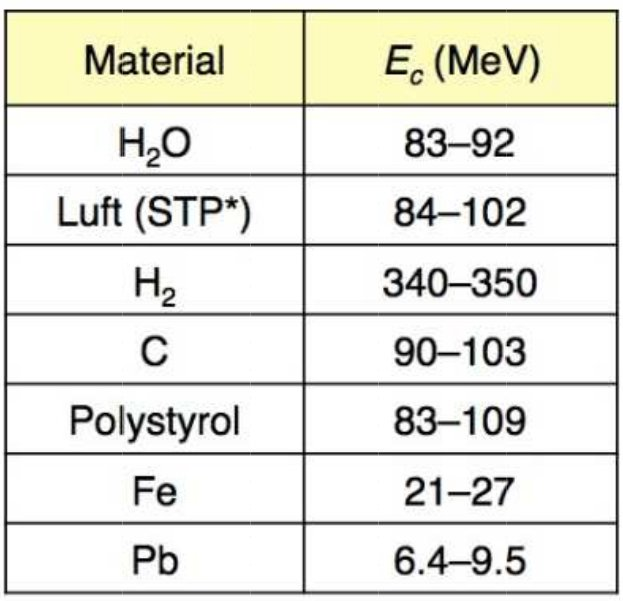
\includegraphics[width=0.5\textwidth]{tabelle1.jpg}
	\caption{}
	\label{}
\end{figure}

\subsubsection*{Strahlungslänge $\chi_0$}

